%\begin{figure}[p]
%    \centering
%    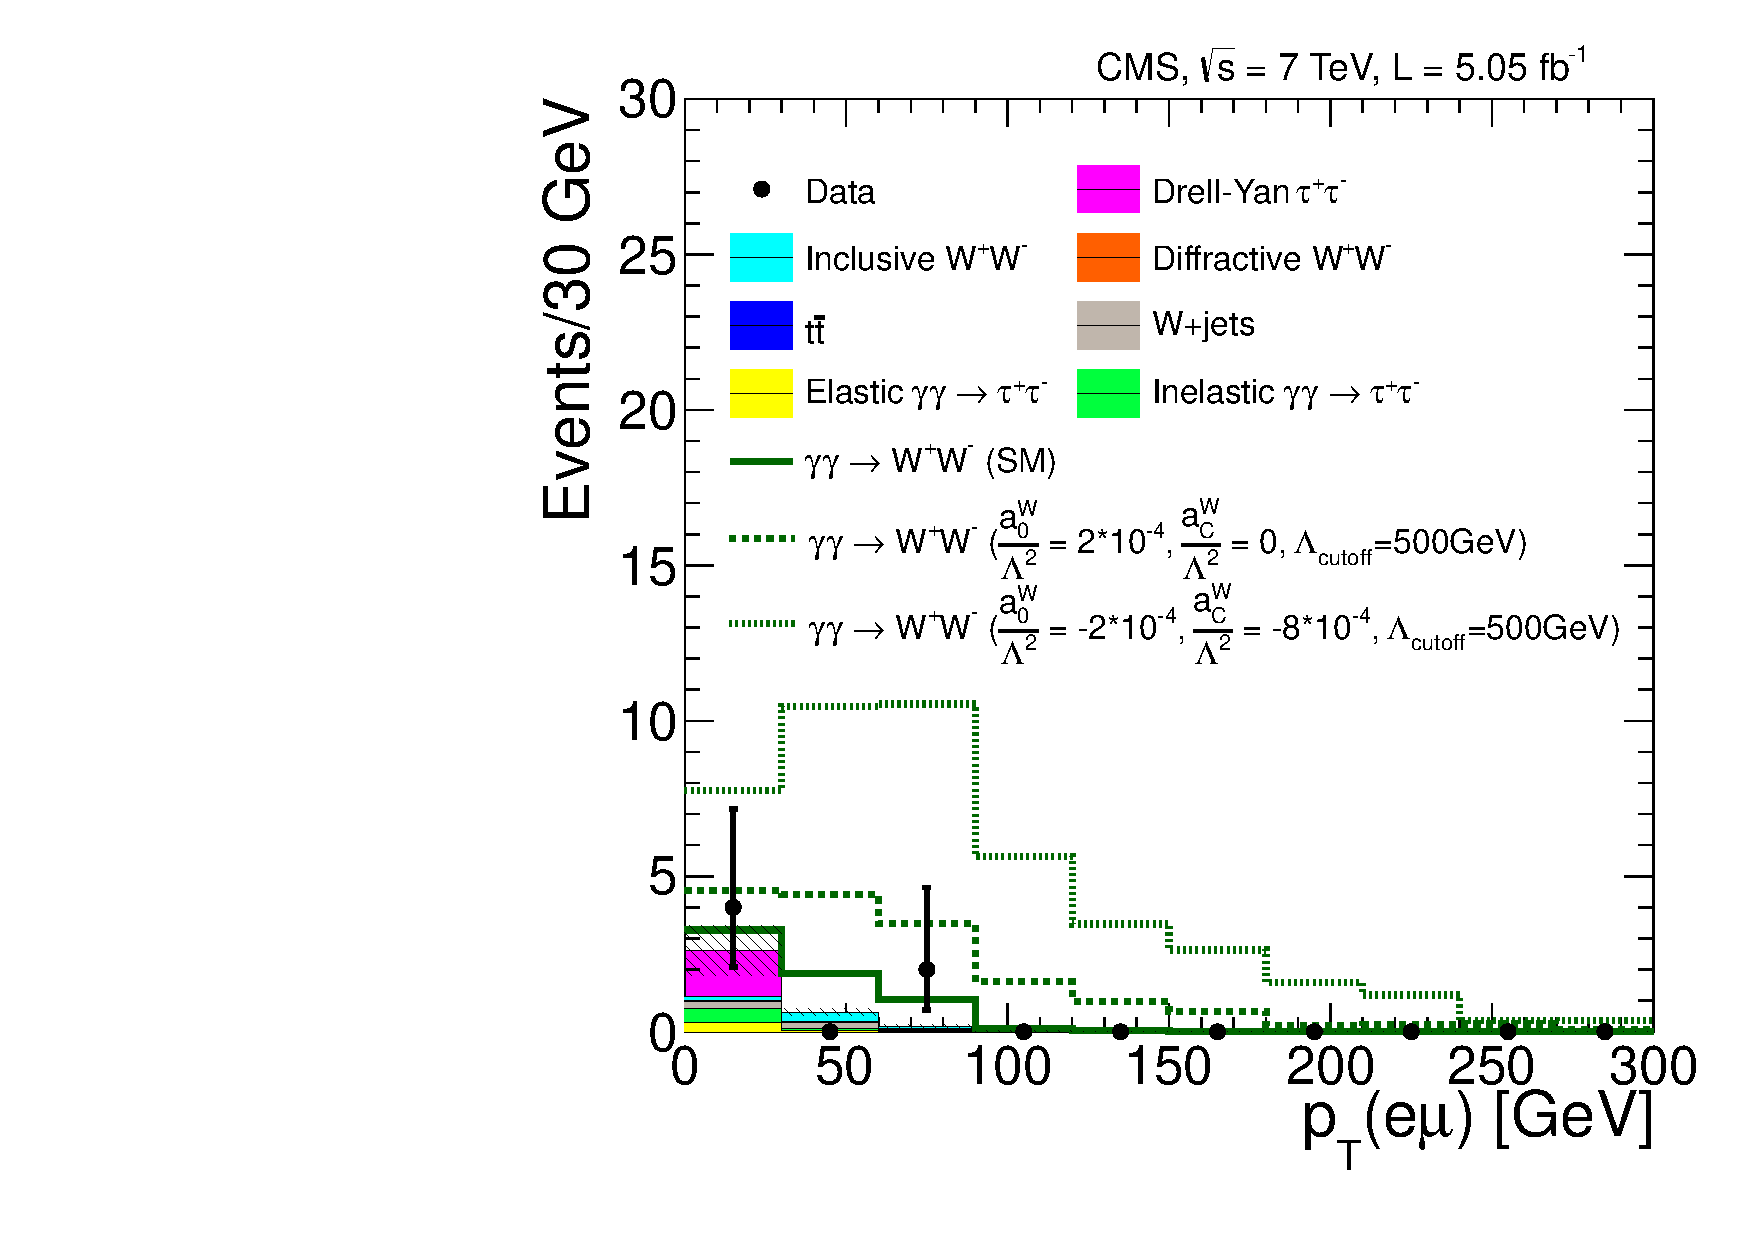
\includegraphics[height=0.3\textheight]{figures/ss-exclboson-ww-cms7tev}
%    \caption{}
%    \label{fig:ss-exclboson-ww-cms7tev}
%\end{figure}
%CMS WWexcl 7 \TeV~\cite{Chatrchyan:2013foa}



\begin{figure}[htb]
\centering
%\includegraphics[width=.48\textwidth]{Figures/2016_01_29_UpdatedPlots/ee_pt.pdf}
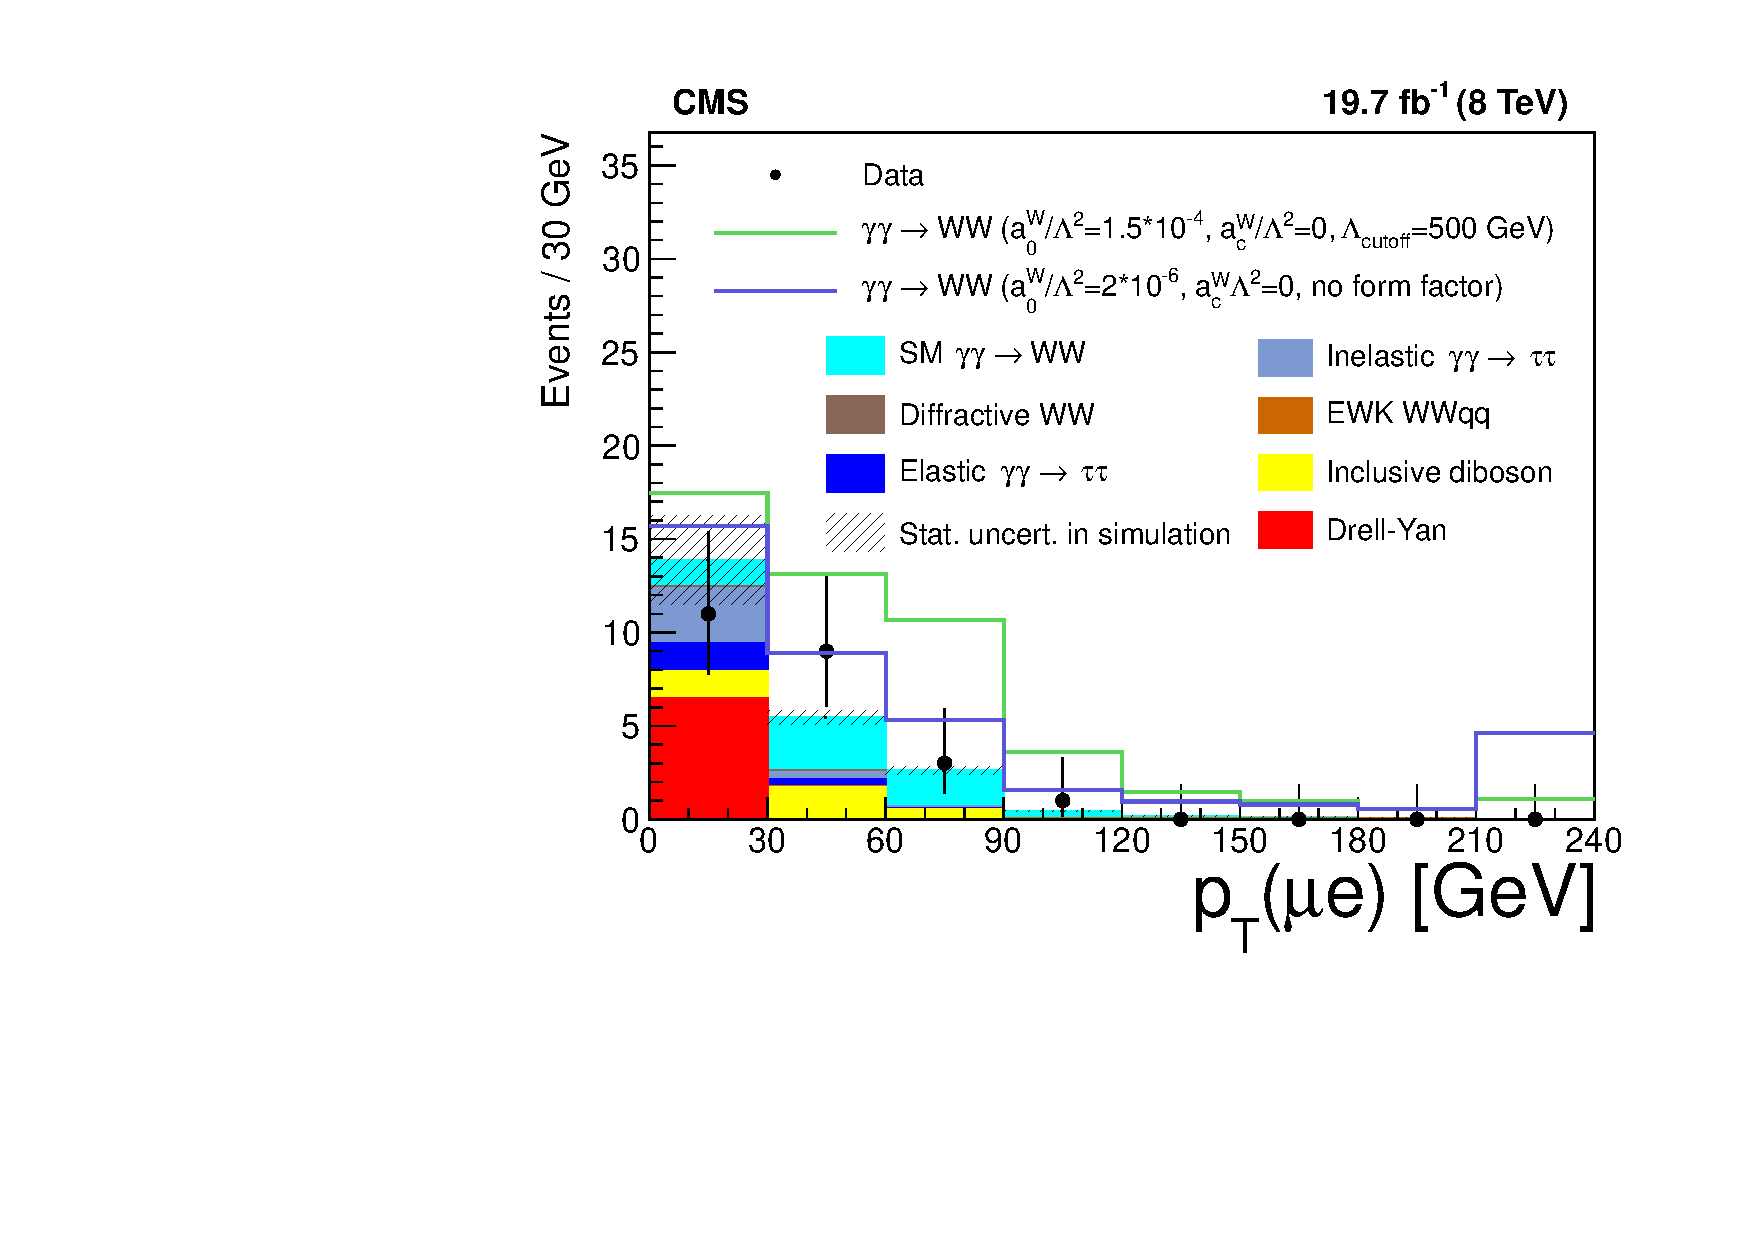
\includegraphics[width=.48\textwidth]{figures/ss-exclboson-ww-cms8tev-1.pdf}
%\includegraphics[width=.48\textwidth]{Figures/2016_01_29_UpdatedPlots/ee_tracks_
%pt30.pdf}
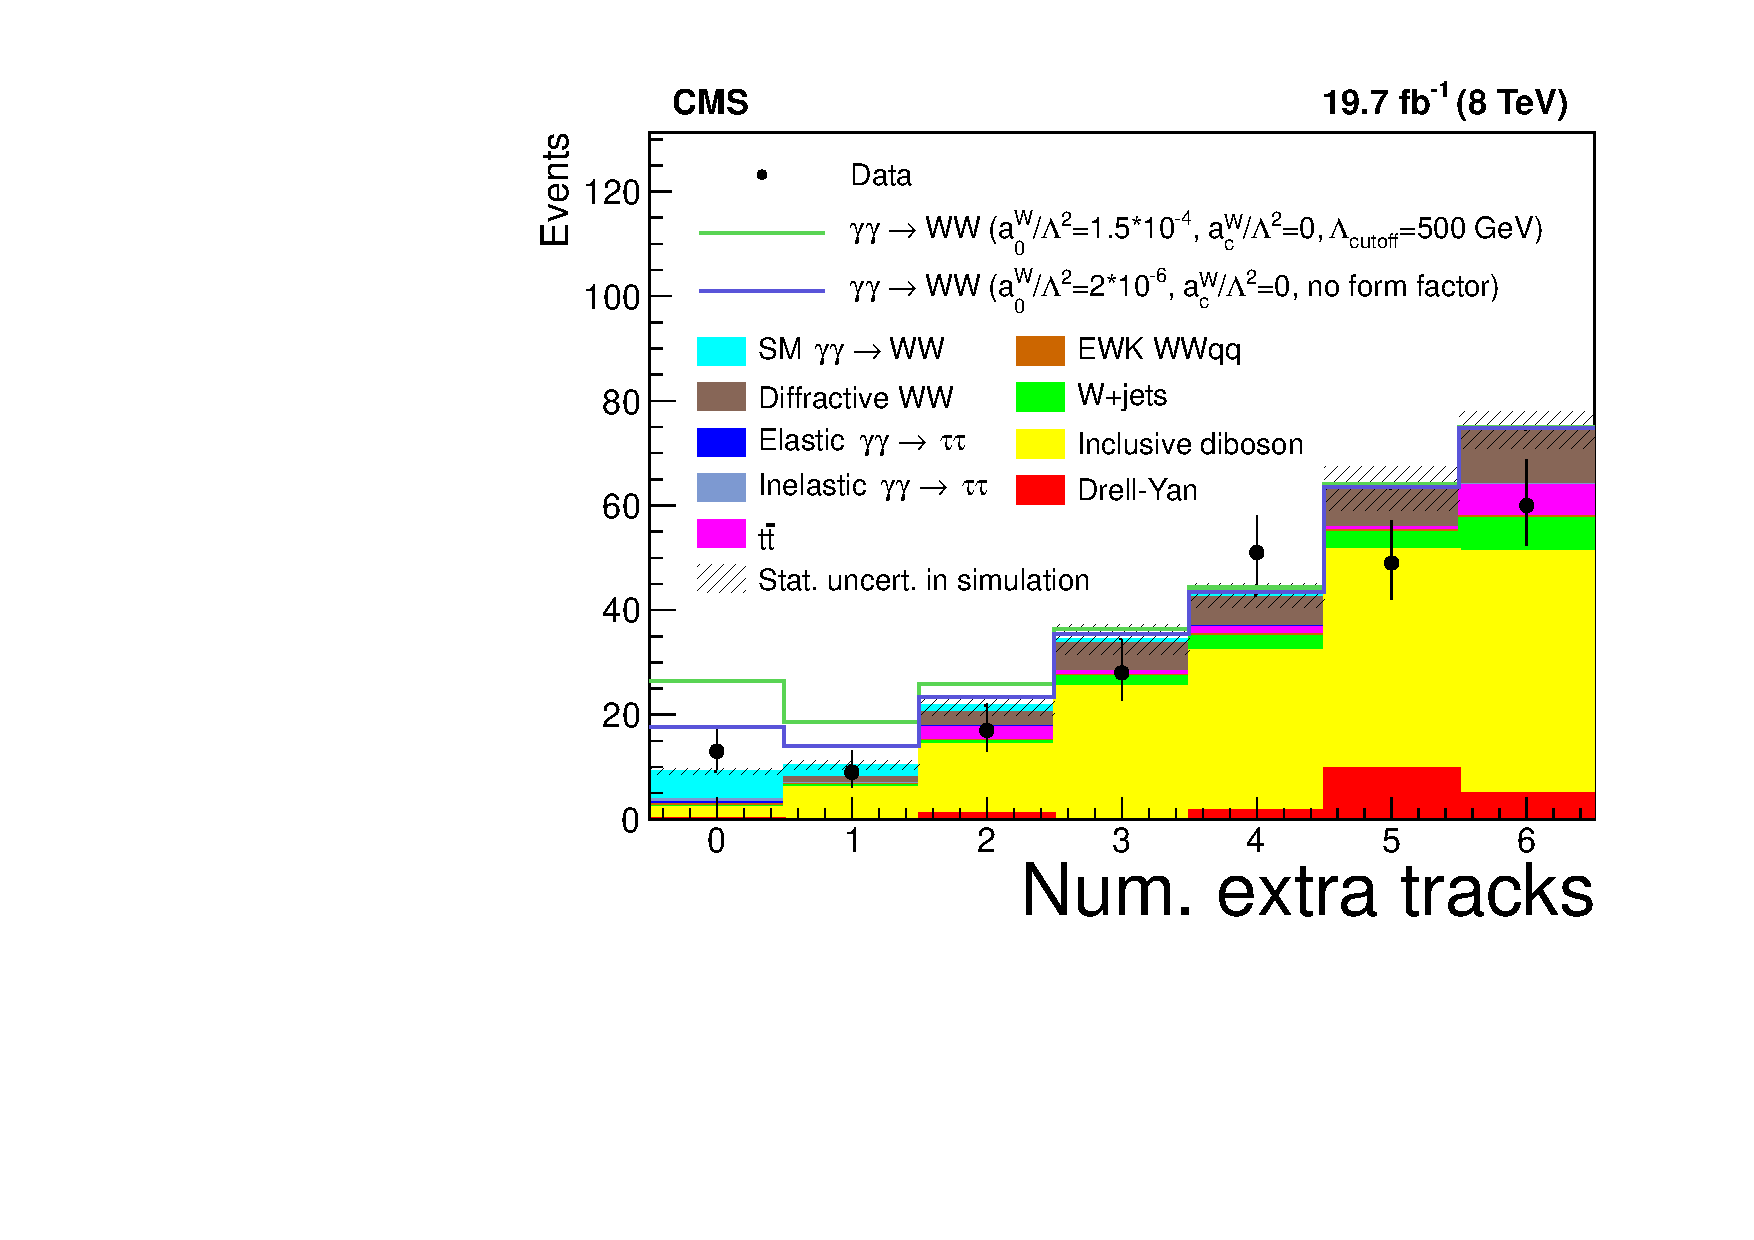
\includegraphics[width=.48\textwidth]{figures/ss-exclboson-ww-cms8tev-2.pdf}
\caption{Evidence for exclusive diboson production via $pp \to p^{(*)}W^+ W^- p^{(*)} \to p^{(*)}\mu^{\pm}e^{\mp}p^{(*)}$.
Distributions of muon-electron transverse momentum for events with zero
 associated tracks (left), and extra-tracks multiplicity for events with $\pt(\mu^{\pm}e^{\mp}) > 30$\GeV (right).
 The data are shown by the points with error bars; the histograms indicate the expected SM signal and backgrounds.
\label{fig:ss-exclboson-ww-cms8tev}}
\end{figure}


\begin{figure*}[htb] {
\centering
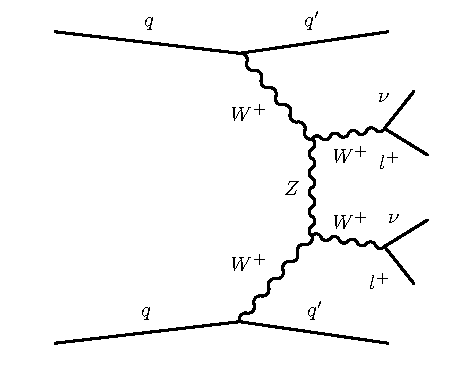
\includegraphics[width=0.315\textwidth]{figures/ss-exclboson-ww-diagram1.pdf}
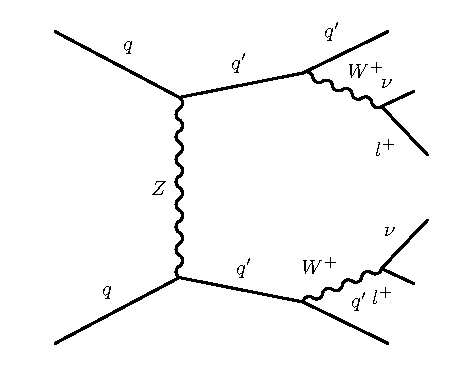
\includegraphics[width=0.35\textwidth]{figures/ss-exclboson-ww-diagram2.pdf}
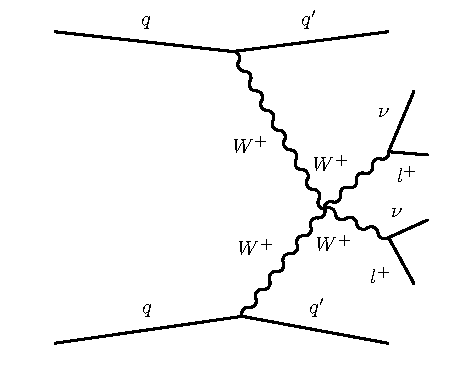
\includegraphics[width=0.315\textwidth]{figures/ss-exclboson-ww-diagram3.pdf}
\caption{
Representative Feynman diagrams for same-sign $WW$ production in association
with two jets from purely electroweak contributions:
(left) vector boson fusion,
(middle) bremsstrahlung-like,
and (right) multiperipheral production.
\label{fig:ss-exclboson-ww-sigdiagram}}

}
\end{figure*}


\begin{figure}[p]
    \centering
    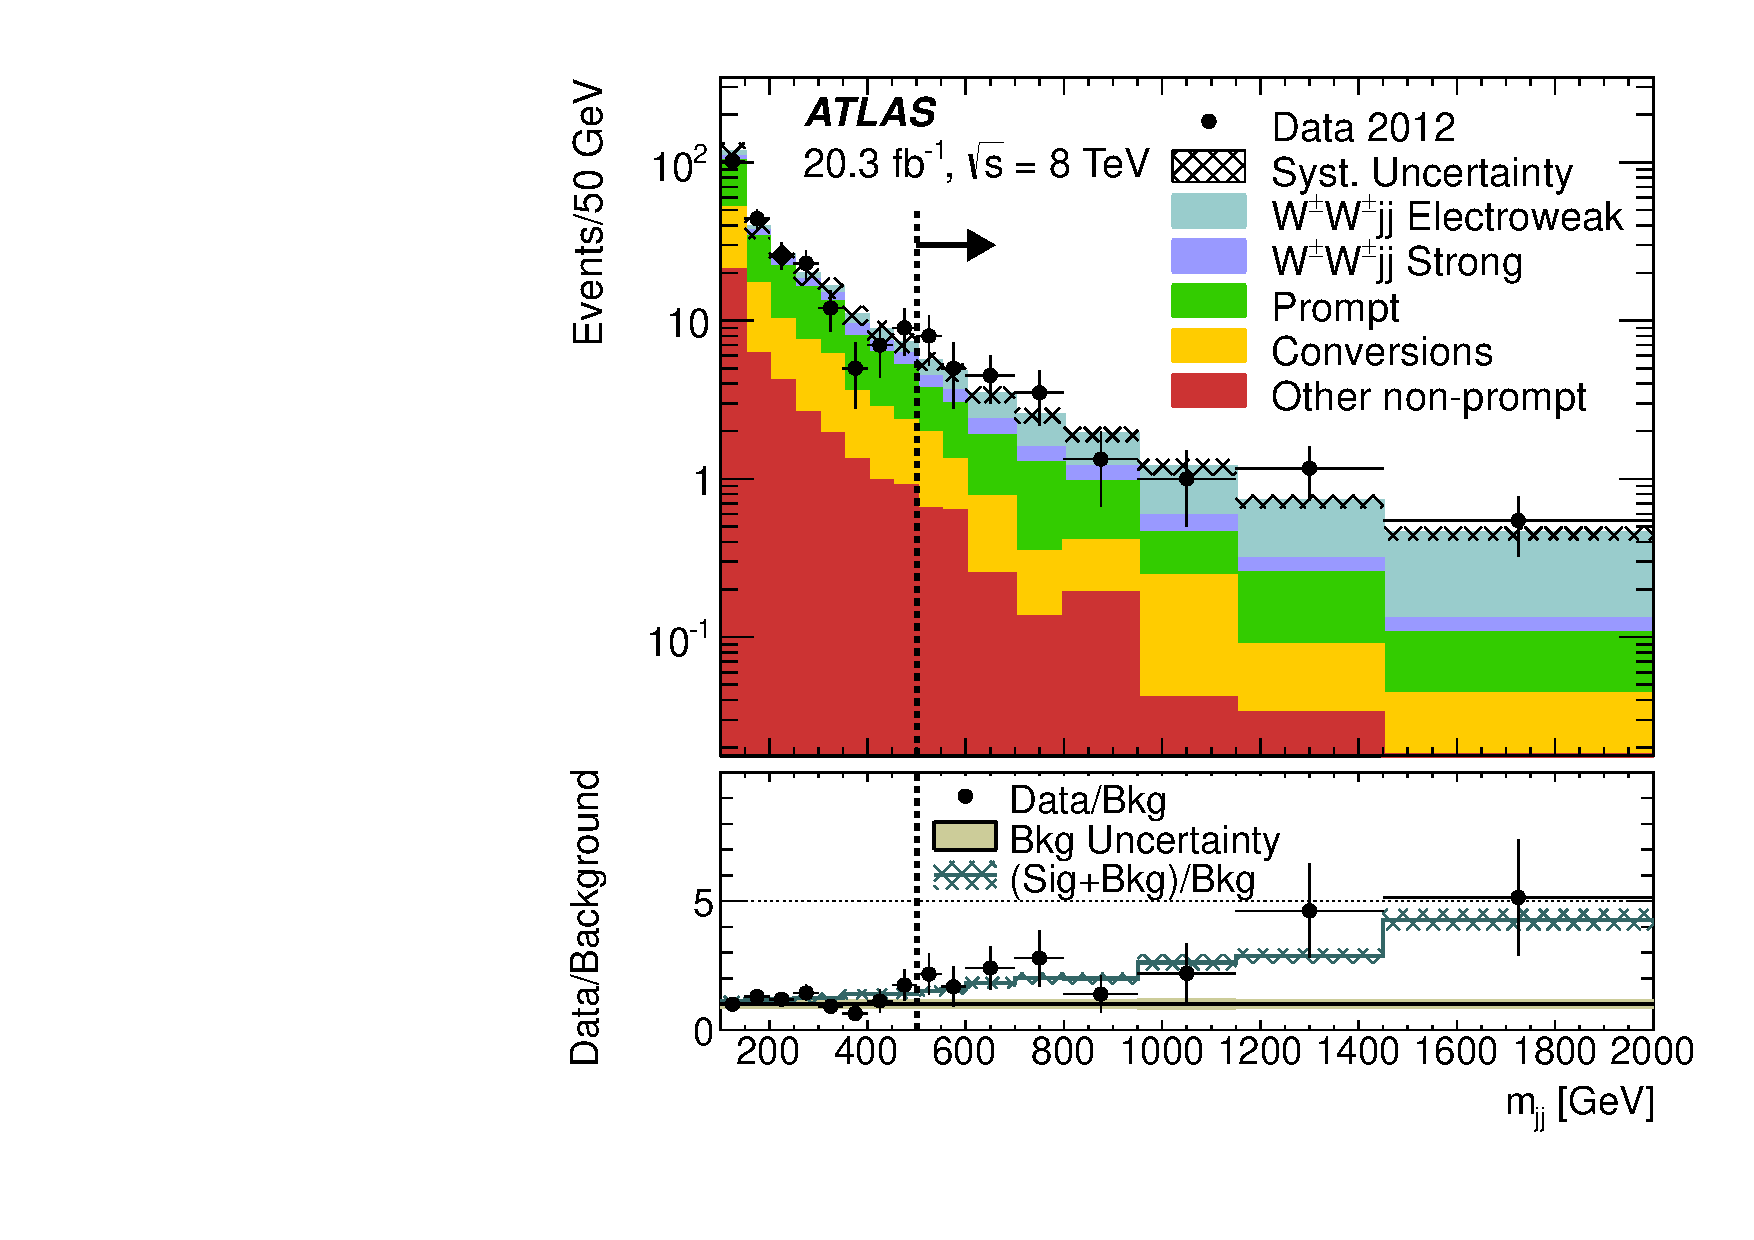
\includegraphics[width=0.45\textwidth]{figures/ss-exclboson-ww-ss-atlas8tev.pdf}
    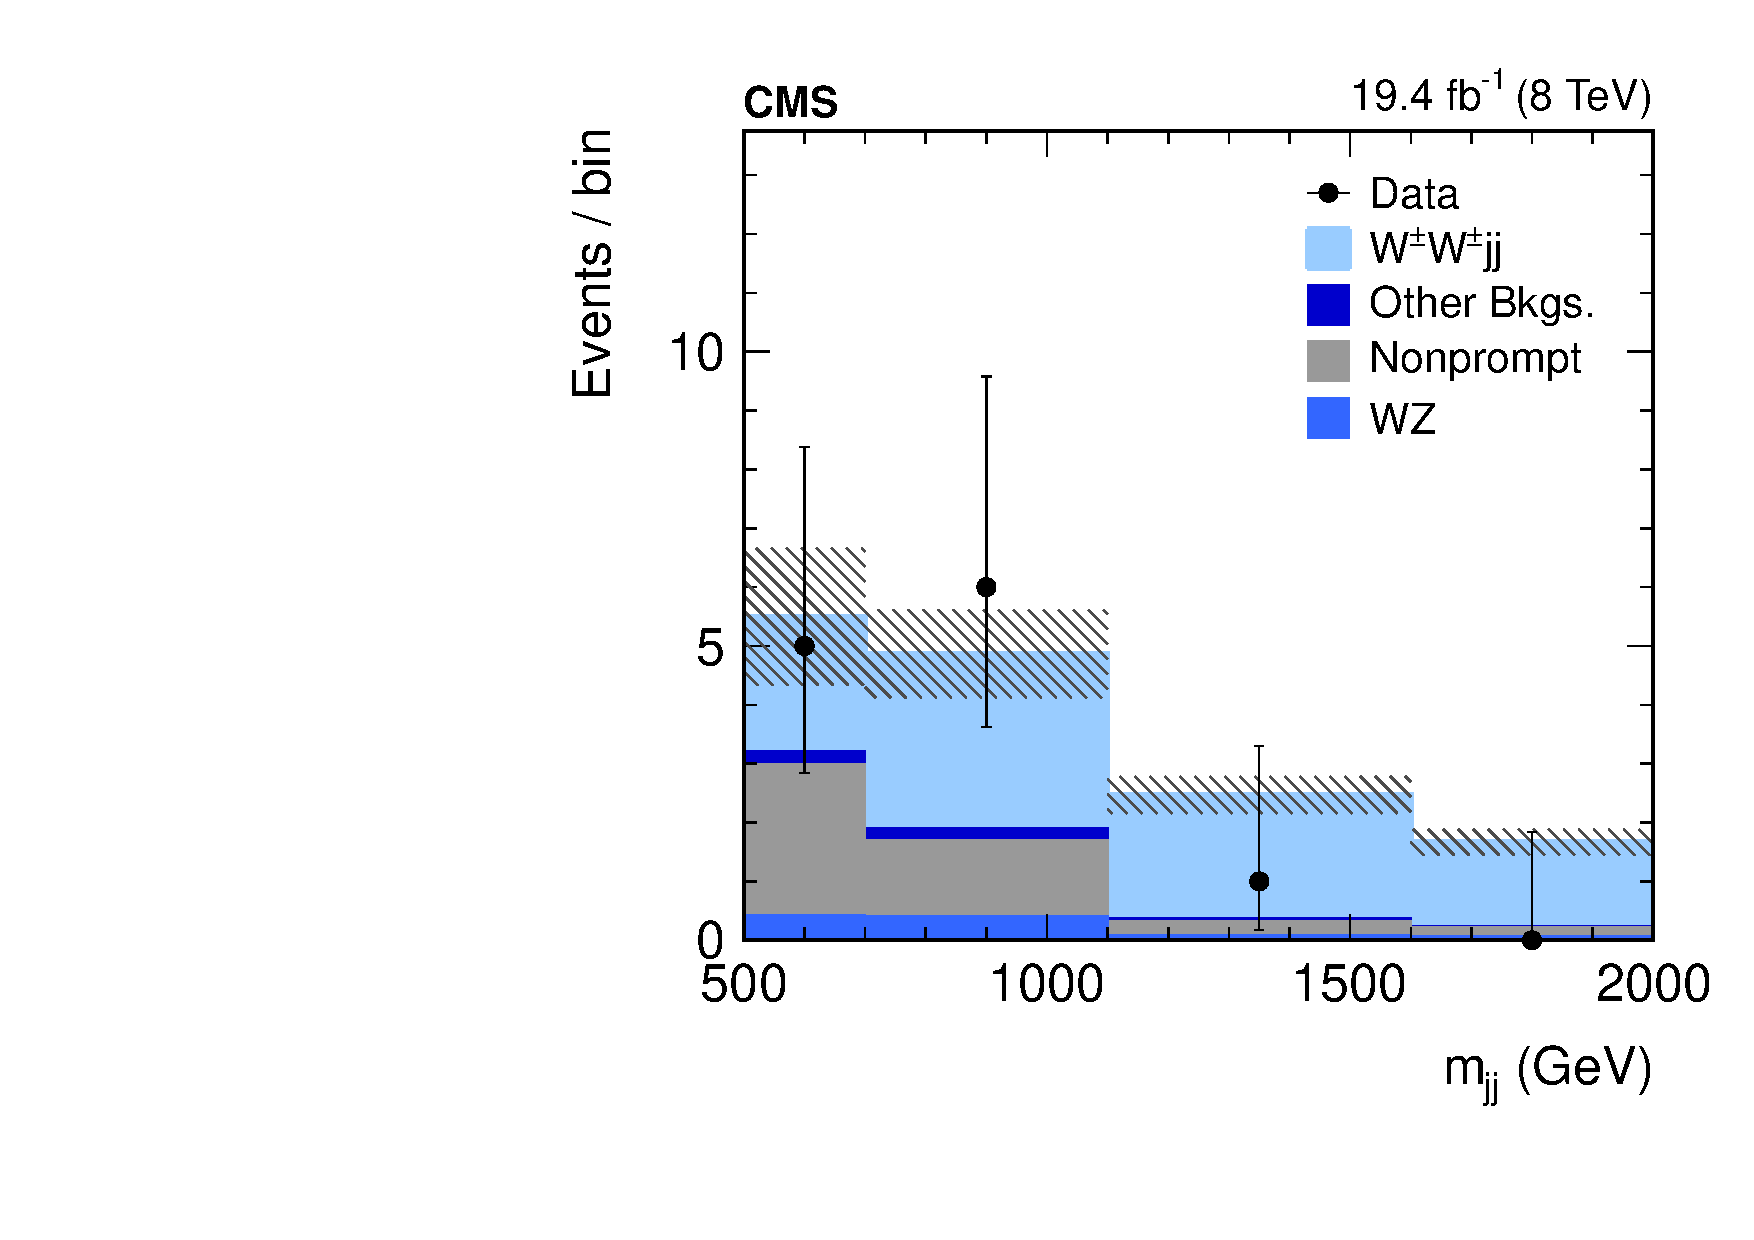
\includegraphics[width=0.45\textwidth]{figures/ss-exclboson-ww-ss-cms8tev.pdf}
    \caption{
    Left:  a signal region by ATLAS.
    Right:  }
    \label{fig:ss-exclboson-ww-ss}
\end{figure}
ATLAS SSWW 8 \TeV~\cite{Aad:2014zda}
CMS SSWW 8 \TeV~\cite{Khachatryan:2014sta}
